Organize this section according to the rules defined in the project description. \\ 

\subsection{External Interface Requirements}

\subsubsection{User Interfaces}
Here will go wireframes
\subsubsection{Hardware Interfaces}
Both users and store managers can use the application through a mobile phone or a personal computer. Users unable to do so will use totems provided by stores.
\subsubsection{Software Interfaces}
map API\\
send ticket/booking requests to CLup\\
send turnstile entrances/exits to CLup\\
query automatically generated reports and obtain their statistics\\
\subsubsection{Communication Interfaces}
The only type of communication required by CLup is a stable internet connection.
\subsection{Functional Requirements}

\subsubsection{List of requirements}
\begin{table}[H]
\label{tab: ReqList}
\begin{tabular}{l|l}
	R1 & Every user can generate a quick ticket for any store \\
	R2 & \pbox{13cm}{Whenever user makes initiates a booking procedure, CLup must be able to compute a suggested least crowded time slot based on historical data} \\
	R3 & \pbox{13cm}{CLup must elaborate and upload data about current global customer affluence to the store during use} \\
	R4 & CLup must admit only valid QR codes for entrance \\
	R5 & CLup must allow users to know current queue status \\
	R6 & CLup must update user on tickets' validity change \\
	R7 & CLup must inform offline users about new tickets (un)availability \\
	R8 & CLup must allow users to indicate which product category they are going to purchase while booking \\
	R9 & CLup must suggest alternative stores when the combination of selected store|time gives no results \\
	R10 & CLup must reserve a non null number of paper tickets at any time for offline customers use 	\\
	R11 & CLup must gather all stores' data about entrance fluxes \\
	R12 & CLup is able to cross affluence data of any supermarket\\
	R13 & CLup keeps track of people who book an entrance and don’t come\\
	R14 & CLup allows store managers to stop quick tickets availability \\
	R15 & CLup is able to generate QR codes\\
	R16 & CLup is able to authenticate users\\
	R17 & CLup is able to store users’ data \\
	R18 & CLup is able to process users' data \\
	R19 & CLup makes quick ticket invalid after 15 minutes delay\\
	R20 & CLup can use stores’ data to sort every store by crowdedness \\
	R21 & Users can see available day/time slots of a supermarket through CLup\\
	R22 & CLup shows to store managers flux data about their supermarket (forse questo è quello che intendeva R3)\\
	R23 & CLup must be able to process reservations\\
	
\end{tabular}
\caption{Requirements list}
\end{table}

\subsubsection{Mapping}
\begin{table} [H]
	\begin{tabular}{c|c|c}
		\textbf{Goals} & \textbf{Requirements} & \textbf{Domain Assumptions}\\
		\hline
		\textbf{G1} & R1, R6, R7, R10, R15,R23 & D1,D5,D8\\
		\hline
		\textbf{G2} & R2, R11, R12, R18, R21 & D1, D2, D8, D10\\
		\hline
		\textbf{G3} & R9, R13, R15, R21, R23 & D5, D8, D10\\
		\hline
		\textbf{G4} & R3, R11, R22 & D1, D2, D8, D11\\
		\hline
		\textbf{G5} & R4, R6, R13, R15, R19 & D1, D2, D3, D8, D10, D11\\
		\hline
		\textbf{G6} & R1, R2, R5, R6 & D4, D5, D6, D7, D8, D10\\
		\hline
		\textbf{G7} & R1, R5, R6, R7, R9, R10, R20, R21, R23 & D2, D4, D5, D8, D9, D10\\
		\hline
		\textbf{G8} & R1, R7, R10 & D6, D7, D8, D10\\
		\hline
		\textbf{G9} & R3, R11, R12, R20 & D1, D2, D8, D9, D10, D11\\
		\hline
		\textbf{G10} & R2, R3, R4, R11, R12, R20 & D1, D2, D3, D7, D8, D10, D11\\
	\end{tabular}
	\caption{Goal mapping summary}
	\label{tab:MappingSum}
\end{table}

\begin{table}[H]
	\rowcolors{1}{white}{white}
	\begin{tabular}{c|l}
		\cellcolor{lightgray}\textbf{G1} & \pbox{13cm}{\textbf{Anybody is guaranteed possibility to make shopping at any supermarket in reasonable time (def. reasonable)}}\\
		\hline
		\cellcolor{YellowGreen} R1 & Every user can generate a quick ticket for any store\\
		\hline
		\cellcolor{YellowGreen} R6 & CLup must update user on tickets' validity change\\
		\hline
		\cellcolor{YellowGreen} R7 & CLup must inform offline users about new tickets (un)availability \\
		\hline
		\cellcolor{YellowGreen} R10 & CLup must reserve a non null number of paper tickets at any time for offline customers use\\
		\hline
		\cellcolor{YellowGreen} R15 & CLup is able to generate QR codes\\
		\hline
		\cellcolor{YellowGreen} R23 & CLup must be able to process reservations\\
		\hline
		\cellcolor{YellowOrange} D1 & Accesses to the store can be monitored\\
		\hline
		\cellcolor{YellowOrange} D5 & Users can estimate the time required to arrive to the store\\
		\hline
		\cellcolor{YellowOrange} D8 & Malicious users are not enough in number or coordination to prevent Clup to work\\
	\end{tabular}
	\label{tab:G1Mapping}
	\caption{G1 Mapping}
\end{table}

\begin{table}[H]
	\rowcolors{1}{white}{white}
	\begin{tabular}{c|l}
		\cellcolor{lightgray}\textbf{G2} & \textbf{Users can get to know the least crowded time slots}\\
		\hline
		\cellcolor{YellowGreen} R2 & \pbox{13cm}{Whenever user makes initiates a booking procedure, CLup must be able to compute a suggested least crowded time slot based on historical data}\\
		\hline
		\cellcolor{YellowGreen} R11 & CLup must gather all stores' data about entrance fluxes\\
		\hline
		\cellcolor{YellowGreen} R12 & CLup is able to cross affluence data of any supermarket\\
		\hline
		\cellcolor{YellowGreen} R18 & CLup is able to process users' data \\
		\hline
		\cellcolor{YellowGreen} R21 & Users can see available day/time slots of a supermarket through CLup\\
		\hline
		\cellcolor{YellowOrange} D1 & Accesses to the store can be monitored\\
		\hline
		\cellcolor{YellowOrange} D2 & Exits from the store can be monitored\\
		\hline
		\cellcolor{YellowOrange} D8 & Malicious users are not enough in number or coordination to prevent Clup to work\\
		\hline
		\cellcolor{YellowOrange} D10 & Store managers give the right information about supermarkets\\
	\end{tabular}
	\label{tab:G2Mapping}
	\caption{G2 Mapping}
\end{table}

\begin{table}[H]
	\rowcolors{1}{white}{white}
	\begin{tabular}{c|l}
		\cellcolor{lightgray}\textbf{G3} & \textbf{Fair users can make a reservation to enter in a supermarket}\\
		\hline
		\cellcolor{YellowGreen} R9 & CLup must suggest alternative stores when the combination of selected store|time gives no results\\
		\hline
		\cellcolor{YellowGreen} R13 & CLup keeps track of people who book an entrance and don’t come\\
		\hline
		\cellcolor{YellowGreen} R15 & CLup is able to generate QR codes \\
		\hline
		\cellcolor{YellowGreen} R21 & Users can see available day/time slots of a supermarket through CLup\\
		\hline
		\cellcolor{YellowGreen} R23 & CLup must be able to process reservations\\
		\hline
		\cellcolor{YellowOrange} D5 & Users can estimate the time required to arrive to the store\\
		\hline
		\cellcolor{YellowOrange} D8 & Malicious users are not enough in number or coordination to prevent Clup to work\\
		\hline
		\cellcolor{YellowOrange} D10 & Store managers give the right information about supermarkets\\
	\end{tabular}
	\label{tab:G3Mapping}
	\caption{G3 Mapping}
\end{table}

\begin{table}[H]
	\rowcolors{1}{white}{white}
	\begin{tabular}{c|l}
		\cellcolor{lightgray}\textbf{G4} & \textbf{Stores can easily monitor fluxes}\\
		\hline
		\cellcolor{YellowGreen} R3 & CLup must elaborate and upload data about current global customer affluence to the store during use\\
		\hline
		\cellcolor{YellowGreen} R11 & CLup must gather all stores' data about entrance fluxes\\
		\hline
		\cellcolor{YellowGreen} R22 & CLup shows to store managers flux data about their supermarket \\
		\hline
		\cellcolor{YellowOrange} D1 & Accesses to the store can be monitored\\
		\hline
		\cellcolor{YellowOrange} D2 & Exits from the store can be monitored\\
		\hline
		\cellcolor{YellowOrange} D8 & Malicious users are not enough in number or coordination to prevent Clup to work\\
		\hline
		\cellcolor{YellowOrange} D11 & Staff guarantees access control systems operativeness\\
	\end{tabular}
	\label{tab:G4Mapping}
	\caption{G4 Mapping}
\end{table}

\begin{table}[H]
	\rowcolors{1}{white}{white}
	\begin{tabular}{c|l}
		\cellcolor{lightgray}\textbf{G5} & \textbf{Only authorized users can access}\\
		\hline
		\cellcolor{YellowGreen} R4 & CLup must admit only valid QR codes for entrance \\
		\hline
		\cellcolor{YellowGreen} R6 & CLup must update user on tickets' validity change\\
		\hline
		\cellcolor{YellowGreen} R13 & CLup keeps track of people who book an entrance and don’t come\\
		\hline
		\cellcolor{YellowGreen} R15 & CLup is able to generate QR codes\\
		\hline
		\cellcolor{YellowGreen} R19 & CLup makes quick ticket invalid after 15 minutes delay\\
		\hline
		\cellcolor{YellowOrange} D1 & Accesses to the store can be monitored\\
		\hline
		\cellcolor{YellowOrange} D2 & Exits from the store can be monitored\\
		\hline
		\cellcolor{YellowOrange} D3 & One customer per authorization given is allowed in by the Staff\\
		\hline
		\cellcolor{YellowOrange} D8 & Malicious users are not enough in number or coordination to prevent Clup to work\\
		\hline
		\cellcolor{YellowOrange} D10 & Store managers give the right information about supermarkets\\
		\hline
		\cellcolor{YellowOrange} D11 & Staff guarantees access control systems operativeness\\
	\end{tabular}
	\label{tab:G5Mapping}
	\caption{G5 Mapping}
\end{table}

\begin{table}[H]
	\rowcolors{1}{white}{white}
	\begin{tabular}{c|l}
		\cellcolor{lightgray}\textbf{G6} & \textbf{Crowds are dramatically reduced outside supermarket stores}\\
		\hline
		\cellcolor{YellowGreen} R1 & Every user can generate a quick ticket for any store\\
		\hline
		\cellcolor{YellowGreen} R2 & \pbox{15cm}{Whenever user makes initiates a booking procedure, CLup must be able to compute a suggested least crowded time slot based on historical data}  \\
		\hline
		\cellcolor{YellowGreen} R5 & CLup must allow users to know current queue status\\
		\hline
		\cellcolor{YellowGreen} R6 & CLup must update user on tickets' validity change\\
		\hline
		\cellcolor{YellowOrange} D4 & Users are reasonably able to manage their time while following the queue evolution\\
		\hline
		\cellcolor{YellowOrange} D5 & Users can estimate the time required to arrive to the store\\
		\hline
		\cellcolor{YellowOrange} D6 & Users who arrives too early at the supermarket don't wait in front of the entrance\\
		\hline
		\cellcolor{YellowOrange} D7 & Customers keep the safe distance\\
		\hline
		\cellcolor{YellowOrange} D8 & Malicious users are not enough in number or coordination to prevent Clup to work\\
		\hline
		\cellcolor{YellowOrange} D10 & Store managers give the right information about supermarkets\\
	\end{tabular}
	\label{tab:G6Mapping}
	\caption{G6 Mapping}
\end{table}

\begin{table}[H]
	\rowcolors{1}{white}{white}
	\begin{tabular}{c|l}
		\cellcolor{lightgray}\textbf{G7} & \pbox{13cm}{\textbf{CLup should not decrease customer affluence beyond a reasonable level w.r.t. to normal (→ define reasonable)}}\\
		\hline
		\cellcolor{YellowGreen} R1 & Every user can generate a quick ticket for any store\\
		\hline
		\cellcolor{YellowGreen} R5 & CLup must allow users to know current queue status\\
		\hline
		\cellcolor{YellowGreen} R6 & CLup must update user on tickets' validity change\\
		\hline
		\cellcolor{YellowGreen} R7 & CLup must inform offline users about new tickets (un)availability \\
		\hline
		\cellcolor{YellowGreen} R9 & CLup must suggest alternative stores when the combination of selected store|time gives no results \\
		\hline
		\cellcolor{YellowGreen} R10 & CLup must reserve a non null number of paper tickets at any time for offline customers use\\
		\hline
		\cellcolor{YellowGreen} R20 & CLup can use stores’ data to sort every store by crowdedness\\
		\hline
		\cellcolor{YellowGreen} R21 & Users can see available day/time slots of a supermarket through CLup\\
		\hline
		\cellcolor{YellowGreen} R23 & CLup must be able to process reservations\\
		\hline
		\cellcolor{YellowOrange} D2 & Exits from the store can be monitored\\
		\hline
		\cellcolor{YellowOrange} D4 & Users are reasonably able to manage their time while following the queue evolution\\
		\hline
		\cellcolor{YellowOrange} D5 & Users can estimate the time required to arrive to the store\\
		\hline
		\cellcolor{YellowOrange} D8 & Malicious users are not enough in number or coordination to prevent Clup to work\\
		\cellcolor{YellowOrange} D9 & Users insert the right starting location or their GPS works\\
		\hline
		\cellcolor{YellowOrange} D10 & Store managers give the right information about supermarkets\\
		\hline
	\end{tabular}
	\label{tab:G7Mapping}
	\caption{G7 Mapping}
\end{table}

\begin{table}[H]
	\rowcolors{1}{white}{white}
	\begin{tabular}{c|l}
		\cellcolor{lightgray}\textbf{G8} & \textbf{Same shopping capabilities guaranteed to offline users}\\
		\hline
		\cellcolor{YellowGreen} R1 & Every user can generate a quick ticket for any store\\
		\hline
		\cellcolor{YellowGreen} R7 & CLup must inform offline users about new tickets (un)availability \\
		\hline
		\cellcolor{YellowGreen} R10 & CLup must reserve a non null number of paper tickets at any time for offline customers use\\
		\hline
		\cellcolor{YellowOrange} D6 & Users who arrives too early at the supermarket don't wait in front of the entrance\\
		\hline
		\cellcolor{YellowOrange} D7 & Customers keep the safe distance\\
		\hline
		\cellcolor{YellowOrange} D8 & Malicious users are not enough in number or coordination to prevent Clup to work\\
		\hline
		\cellcolor{YellowOrange} D7 & Customers keep the safe distance\\
	\end{tabular}
	\label{tab:G8Mapping}
	\caption{G8 Mapping}
\end{table}

\begin{table}[H]
	\rowcolors{1}{white}{white}
	\begin{tabular}{c|l}
		\cellcolor{lightgray}\textbf{G9} & \pbox{13cm}{\textbf{Find the best (less crowded, soonest available) alternative among local supermarket stores (of same franchise only?)}}\\
		\hline
		\cellcolor{YellowGreen} R3 & CLup must elaborate and upload data about current global customer affluence to the store during use \\
		\hline
		\cellcolor{YellowGreen} R11 & CLup must gather all stores' data about entrance fluxes \\
		\hline
		\cellcolor{YellowGreen} R12 & CLup is able to cross affluence data of any supermarket\\
		\hline
		\cellcolor{YellowGreen} R20 & CLup can use stores’ data to sort every store by crowdedness\\
		\hline
		\cellcolor{YellowOrange} D1 & Accesses to the store can be monitored\\
		\hline
		\cellcolor{YellowOrange} D2 & Exits from the store can be monitored\\
		\hline
		\cellcolor{YellowOrange} D8 & Malicious users are not enough in number or coordination to prevent Clup to work\\
		\hline
		\cellcolor{YellowOrange} D9 & Users insert the right starting location or their GPS works\\
		\hline
		\cellcolor{YellowOrange} D10 & Store managers give the right information about supermarkets\\
		\hline
		\cellcolor{YellowOrange} D11 & Staff guarantees access control systems operativeness\\
	\end{tabular}
	\label{tab:G9Mapping}
	\caption{G9 Mapping}
\end{table}

\begin{table}[H]
	\rowcolors{1}{white}{white}
	\begin{tabular}{c|l}
		\cellcolor{lightgray}\textbf{G10} & \pbox{13cm}{\textbf{Supermarkets do not overcrowd}}\\
		\hline
		\cellcolor{YellowGreen} R2 & \pbox{13cm}{Whenever user makes initiates a booking procedure, CLup must be able to compute a suggested least crowded time slot based on historical data} \\
		\hline
		\cellcolor{YellowGreen} R3 & CLup must elaborate and upload data about current global customer affluence to the store during use\\
		\hline
		\cellcolor{YellowGreen} R4 & CLup must admit only valid QR codes for entrance\\
		\hline
		\cellcolor{YellowGreen} R11 & CLup must gather all stores' data about entrance fluxes\\
		\hline
		\cellcolor{YellowGreen} R12 & CLup is able to cross affluence data of any supermarket\\
		\hline
		\cellcolor{YellowGreen} R20 & CLup can use stores’ data to sort every store by crowdedness\\
		\hline
		\cellcolor{YellowOrange} D1 & Accesses to the store can be monitored\\
		\hline
		\cellcolor{YellowOrange} D2 & Exits from the store can be monitored\\
		\hline
		\cellcolor{YellowOrange} D3 & One customer per authorization given is allowed in by the Staff\\
		\hline
		\cellcolor{YellowOrange} D7 & Customers keep the safe distance\\
		\hline
		\cellcolor{YellowOrange} D8 & Malicious users are not enough in number or coordination to prevent Clup to work\\
		\hline
		\cellcolor{YellowOrange} D10 & Store managers give the right information about supermarkets\\
		\hline
		\cellcolor{YellowOrange} D11 & Staff guarantees access control systems operativeness\\
	\end{tabular}
	\label{tab:G10Mapping}
	\caption{G10 Mapping}
\end{table}

\subsubsection{Use cases}

\begin{enumerate}
	
%TABELLA 1
\item \textbf{Registration of new account}

\begin{table}[H]
{\rowcolors{1}{white}{white}
\begin{tabular}{|c|p{14cm}|}
	\hline
	Name & Registration of new account\\
	\hline
	Actors & User\\
	\hline
	Entry Condition & User installed and opened the app and doesn’t have an account or wants to register another one\\
	\hline
	Event Flow & \begin{enumerate}
		\item User opens the app.
		\item Login screen loads.
		\item User taps “Sign up".
		\item TODO REGISTRATION WIREFRAME.
		\end{enumerate}\\
	\hline
	Exit Conditions & User now has an account with which he can log in\\
	\hline
	Exception & \begin{enumerate}
		\item There is no internet when the user presses “create account”
	\end{enumerate}
	
	“No internet” popup, the user can either wait for internet to come back or discard the incomplete account creation by going back to main screen\\
	\hline
\end{tabular}
}
	\label{tab:UCRegister}
	\caption{Use case: User registration}
\end{table}

%TABELLA 2
\item \textbf{User login}
	
\begin{table}[H]
{\rowcolors{1}{white}{white}
	\begin{tabular}{|c|p{14cm}|}
		\hline
		Name & User login\\
		\hline
		Actors & User\\
		\hline
		Entry Condition & User already has an account\\
		\hline
		Event Flow & \begin{enumerate}
			\item User opens the app.
			\item Login screen loads.
			\item User already has an account.
			\item User inputs his credentials and presses “login”
			\item Main screen loads
		\end{enumerate}\\
		\hline
		Exit Conditions & User logged in and is now in main screen, from where he can virtually access all of the app’s functionalities\\
		\hline
		Exception & \begin{enumerate}
			\item Credentials are wrong\newline
			wrong credentials popup, user stays in  login screen
			
			\item There is no internet connection\newline
			no internet warning pop up, user still logs in if he used previously inserted and saved credentials so he can still edit settings and filters or look at his history 
			
		\end{enumerate}\\
		
		\hline
	\end{tabular}
}
	\label{tab:UCLogin}
	\caption{Use case: User login}
\end{table}

%TABELLA 3
\item \textbf{Quick ticket request}
	
\begin{table}[H]
{\rowcolors{1}{white}{white}
	\begin{tabular}{|c|p{14cm}|}
		\hline
		Name & ASAP ticket request\\
		\hline
		Actors & User\\
		\hline
		Entry Condition & User successfully logged in and is in main screen\\
		\hline
		
		Event Flow & \begin{enumerate}
			\item User taps “Show stores”
			\item User is taken to “Quick results” screen
			\item IF LIST MODE (from settings)\newline
			stores with queue time, size and distance are shown in a list according to setted filters, if show more is pressed more stores are loaded and the list is made scrollable, if location button is pressed a map showing the store’s location is shown (TODO browse stores on map)\newline
			IF MAP MODE (from settings\newline)
			stores with queue time, size and distance are shown on a map, if list button is pressed User is taken to the previously descripted “list mode” case
			\item User taps on a store
			\item Confirmation pop up is shown
			\item If user confirms “Ticket screen” is shown, otherwise he is taken back to 3
		\end{enumerate}\\
	
		\hline
		Exit Conditions & User has a ticket with updating due time to enter the store\\
		\hline
		
		Exception & \begin{enumerate}
			\item The store blocked ticket requests\newline
			after 5 user is told that the store is no longer available and remains in list/map to make an eventual different choice
			
			\item There is no internet connection\newline
			after 1 user stays in main screen with a dismissable “no internet” pop up
			
			\item User already has an ASAP ticket\newline
			after 1 user stays in main screen with a dismissable “you can only have one ASAP ticket” 
			
		\end{enumerate}\\
		
		\hline
	\end{tabular}
}
	\label{tab:UCQuick}
	\caption{Use case: Quick ticket request}
\end{table}

%TABELLA 4
\item \textbf{Quick ticket request at physical Totem}

\begin{table}[H]
{\rowcolors{1}{white}{white}
	\begin{tabular}{|c|p{14cm}|}
		\hline
		Name & ASAP ticket request at physical Totem\\
		\hline
		Actors & User\\
		\hline
		Entry Condition & User starts interacting with CLup tablet (?) outside the store\\
		\hline
		
		Event Flow & \begin{enumerate}
			\item POSSIBLE IDENTIFICATION (fiscal code or ID card)
			\item User sees current queue for this store and decides whether to confirm or cancel
			\item A card ticket with remainder and QR is printed
			\item User leaves the station with his printed ticket
			
		\end{enumerate}\\
		
		\hline
		Exit Conditions & User has a ticket that he can scan to enter the store when he comes back at the written date and time\\
		\hline
		
		Exception & \begin{enumerate}
			\item The store blocked ticket requests\newline
			User can’t get a ticket and is asked to come back another time
			
		\end{enumerate}\\
		
		\hline
	\end{tabular}
}
	\label{tab:UCTotem}
	\caption{Use case: Quick ticket at physical totem}
\end{table}

%TABELLA 5
\item \textbf{Edit filters}

\begin{table}[H]
{\rowcolors{1}{white}{white}
	\begin{tabular}{|c|p{14cm}|}
		\hline
		Name & Edit filters\\
		\hline
		Actors & User\\
		\hline
		Entry Condition & User pressed filter button from main screen\\
		\hline
		
		Event Flow & \begin{enumerate}
			\item User is in main screen and taps the “filters” button
			\item User is in filters screen
			\item User changes the filter parameters he wants to change among:
			\begin{enumerate}
				\item distance range
				\item store type
				\item default booking time (ignored by ticket request)
				\item default calendar or stores first when booking (ignored by ticket request)
				\item default map or list view when booking (ignored by ticket request)
				\item ???
			\end{enumerate}
			
			\item User presses back to main screen button
			\item Popup to confirm and save or discard the new filters is shown 

		\end{enumerate}\\
		
		\hline
		Exit Conditions & New filters are set and they will affect the next ticket request or visit plan\\
		\hline
	
		Exception & \begin{enumerate}
			\item User closes the app without saving the filters\newline
			Filter modifications are lost
			
		\end{enumerate}\\
		
		\hline
	\end{tabular}
}
	\label{tab:UCEdit}
	\caption{Use case: Edit filters}
\end{table}

%TABELLA 6 
\item \textbf{Plan visit}

\begin{table}[H]
{\rowcolors{1}{white}{white}
	\begin{tabular}{|c|p{14cm}|}
		\hline
		Name & ASAP ticket request\\
		\hline
		Actors & User\\
		\hline
		Entry Condition & User successfully logged in and is in main screen\\
		\hline
		
		Event Flow & \begin{enumerate}
			\item User taps “Show stores”
			\item User is taken to “Quick results”
			\item User inputs the expected amount of time he will be shopping
			\item Calendar or store map/list is shown depending on what was loaded given the filter settings
			\item User chooses date or store (from map/list) 
			\item Stores map/list or calendar depending on what was shown already
			\item User chooses the store or the day
			\item CLup shows time slots for that store on that day
			\item User taps on a time slot
			\item Confirmation pop up is shown
			\item If user confirms “Ticket screen” is shown, otherwise he is taken back to 3			
		\end{enumerate}\\
		
		\hline
		Exit Conditions & User has a ticket with updating due time to enter the store\\
		\hline
		
		Exception & \begin{enumerate}
			\item The store blocked ticket requests\newline
			after 5 user is told that the store is no longer available and remains in list/map to make an eventual different choice
			
			\item There is no internet connection\newline
			after 1 user stays in main screen with a dismissable “no internet” pop up
			
			\item User already has an ASAP ticket\newline
			after 1 user stays in main screen with a dismissable “you can only have one ASAP ticket”
			
			\item Day/store/time slot is full\newline
			the choice is refused with a popup and user has to choose an alternative
			
		\end{enumerate}\\
		
		\hline
	\end{tabular}
}
	\label{tab:UCPlan}
	\caption{Use case: Plan visit}
\end{table}

%TABELLA 7
\item \textbf{Enter store}

\begin{table}[H]
	{\rowcolors{1}{white}{white}
		\begin{tabular}{|c|p{14cm}|}
			\hline
			Name & Enter store\\
			\hline
			Actors & User\\
			\hline
			Entry Condition & User has a valid QR ticket and is at the store entrance\\
			\hline
			
			Event Flow & \begin{enumerate}
				\item User scans his QR ticket or inputs his alphanumeric code at the turnstile
				\item The turnstile informs the user he can enter and unlocks
				\item The user enters the store
				
			\end{enumerate}\\
			
			\hline
			Exit Conditions & The user is in the store and can start shopping\\
			\hline
			
			Exception & \begin{enumerate}
				\item The ticket expired its 15 minutes validity time\newline
				The turnstile remains locked and informs the user that his ticket is not valid, the ticket expiration causes a report to be generated for the manager independently from the fact that the user tried to enter anyway
				
				\item The code is wrong\newline
				The turnstile remains locked and informs the user that the code is not valid

			\end{enumerate}\\
			
			\hline
		\end{tabular}
	}
	\label{tab:UCEnter}
	\caption{Use case: Enter store}
\end{table}

%TABELLA 8
\item \textbf{Exit store}

\begin{table}[H]
	{\rowcolors{1}{white}{white}
		\begin{tabular}{|c|p{14cm}|}
			\hline
			Name & Exit store\\
			\hline
			Actors & User\\
			\hline
			Entry Condition & User has a valid QR ticket and is exiting the store\\
			\hline
			
			Event Flow & \begin{enumerate}
				\item User scans his QR ticket or inputs his alphanumeric code or inputs his CLup email or nickname at the turnstile
				\item The turnstile informs the user he can exit and unlocks
				\item The user exits the store
				
			\end{enumerate}\\
			
			\hline
			Exit Conditions & The user is in the store and can start shopping\\
			\hline
			
			Exception & \begin{enumerate}
				\item The code is wrong or no code can be provided or credentials are wrong\newline
				The turnstile informs the user that he has to try again and after the third try it is unlocked anyway, the user exit won’t be tracked and will cause a report for the misinterpreted long shopping to be generated for him anyway
				
				
			\end{enumerate}\\
			
			\hline
		\end{tabular}
	}
	\label{tab:UCExit}
	\caption{Use case: Exit store}
\end{table}

%TABELLA 9
\item \textbf{Store manager stops new entrances}

\begin{table}[H]
	{\rowcolors{1}{white}{white}
		\begin{tabular}{|c|p{14cm}|}
			\hline
			Name & Stops new entrances\\
			\hline
			Actors & Store manager\\
			\hline
			Entry Condition & Store manager is in management web page\\
			\hline
			
			Event Flow & \begin{enumerate}
				\item Manager clicks on stop new entrances
				\item Manager is asked to insert admin password
				\item Manager is asked to confirm and he does
				
			\end{enumerate}\\
			
			\hline
			Exit Conditions & No new tickets can be issued and currently released tickets are put on hold, meaning that valid tickets won’t be accepted by the turnstiles (queue time replaced with a suspened entrances message)
			The page now offers the possibility to allow entrances again\\
			\hline
			
			Exception & None\\
			
			\hline
		\end{tabular}
	}
	\label{tab:UCManStop}
	\caption{Use case: Store manager stops new entrances}
\end{table}

%TABELLA 10
\item \textbf{Store manager views affluence statistics}

\begin{table}[H]
	{\rowcolors{1}{white}{white}
		\begin{tabular}{|c|p{14cm}|}
			\hline
			Name & View affluence statistics\\
			\hline
			Actors & Store manager\\
			\hline
			Entry Condition & The manager is in management web page\\
			\hline
			
			Event Flow & \begin{enumerate}
				\item Staff clicks on “View affluence statistics”
				\item A page showing various statistics with customizable filters and options about people affluences is shown
				
			\end{enumerate}\\
			
			\hline
			Exit Conditions & Manager knows their customers’ behaviours (e.g. affluence and permanence times) and can act accordingly\\
			\hline
			
			Exception & \begin{enumerate}
				\item None
				
			\end{enumerate}\\
			
			\hline
		\end{tabular}
	}
	\label{tab:UCStatistic}
	\caption{Use case: Store manager views affluence statistics}
\end{table}

%TABELLA 11
\item \textbf{Store manager changes store capacity}

\begin{table}[H]
	{\rowcolors{1}{white}{white}
		\begin{tabular}{|c|p{14cm}|}
			\hline
			Name & Change store capacity\\
			\hline
			Actors & Store manager\\
			\hline
			Entry Condition & Manager is in management web page\\
			\hline
			
			Event Flow & \begin{enumerate}
				\item Staff clicks on “Change people capacity”
				\item A screen which contains a text box to input the people number for store capacity is shown
				\item Staff inputs the new number and clicks confirm
				\item Admin password is asked to proceed
				\item Confirmation is asked and done
				
				
			\end{enumerate}\\
			
			\hline
			Exit Conditions & The number of people that can be let in the store after scanning their code is now set to the amount desired by the store staff\\
			\hline
			
			Exception & if more people than store capacity are inside no new people will be let in until the store doesn’t empty below the limit, possibly clearing the store is outside of the scope of this project\newline
			\begin{enumerate}
				\item Password is wrong\newline
				no changes are allowed, password is asked again
				
			\end{enumerate}\\
			
			\hline
		\end{tabular}
	}
	\label{tab:UCManCap}
	\caption{Use case: Store manager changes store capacity}
\end{table}

%TABELLA 12
\item \textbf{Store manager inspect reports}

\begin{table}[H]
	{\rowcolors{1}{white}{white}
		\begin{tabular}{|c|p{14cm}|}
			\hline
			Name & Store manager inspect reports\\
			\hline
			Actors & Manager\\
			\hline
			Entry Condition & Manager is in management webpage\\
			\hline
			
			Event Flow & \begin{enumerate}
				\item Manager clicks on “Inspect reports”
				\item Reports page is shown
				\item Manager can navigate the complete list of reports, if complying per store, and can filter or search them 
				
			\end{enumerate}\\
			
			\hline
			Exit Conditions & Manager now knows the users infringements and can take informed actions on blocking or unblocking them from queuing in the stores\\
			\hline
			
			Exception & None (if more people than store capacity are inside no new people will be let in until the store doesn’t empty below the limit)\\
			
			\hline
		\end{tabular}
	}
	\label{tab:UCManReport}
	\caption{Use case: Store manager inspects report}
\end{table}

%TABELLA 13
\item \textbf{Store manager blocks/unblocks user}

\begin{table}[H]
	{\rowcolors{1}{white}{white}
		\begin{tabular}{|c|p{14cm}|}
			\hline
			Name & Store manager blocks/unblocks user\\
			\hline
			Actors & Manager\\
			\hline
			Entry Condition & Manager is in management web page \\
			\hline
			
			Event Flow & \begin{enumerate}
				\item Store staff clicks on “block/unblock user”
				\item Admin password is asked to proceed
				\item A screen with a search box to look for a user and navigate blocked users is shown
				\item Staff looks for the user on which they want to take action
				\item Staff clicks “block” or “unblock” button near the username of the user in question
				\item Admin password is asked to proceed
				
			\end{enumerate}\\
			
			\hline
			Exit Conditions & Chosen user is now blocked or unblocked for queuing at the store\\
			\hline
			
			Exception & \begin{enumerate}
				\item The user doesn’t exist (anymore)\newline
				an error message informs that the action cannot be completed
				
				\item The user is already blocked / unblocked\newline
				an error message informs that the user is already blocked / unblocked
				
				\item Password is wrong\newline
				no changes are allowed, password is asked again
				
			\end{enumerate}\\
			
			\hline
		\end{tabular}
	}
	\label{tab:UCManBlock}
	\caption{Use case: Store manager (un)blocks user}
\end{table}

%TABELLA 14
\item \textbf{Store manager login}

\begin{table}[H]
	{\rowcolors{1}{white}{white}
		\begin{tabular}{|c|p{14cm}|}
			\hline
			Name & Store manager login\\
			\hline
			Actors & Manager\\
			\hline
			Entry Condition & Manager is in management web page\\
			\hline
			
			Event Flow & \begin{enumerate}
				\item Staff opens the CLup website
				\item Staff inserts login store code and password and clicks login button
				
			\end{enumerate}\\
			
			\hline
			Exit Conditions & Staff is now in the management web page main screen\\
			\hline
			
			Exception & \begin{enumerate}
				\item Credentials are wrong\newline
				Error message is shown, it is asked to re insert the credentials
				\item Too many login attempts\newline
				After 3 failed login attempts the login-attempting ip is blocked for some time from trying other logins and if the store code was valid its staff will be notified of the attempt
				
			\end{enumerate}\\
			
			\hline
		\end{tabular}
	}
	\label{tab:UCManLog}
	\caption{Use case: Store manager login}
\end{table}

%TABELLA 15
\item \textbf{Edit filters}

\begin{table}[H]
	{\rowcolors{1}{white}{white}
		\begin{tabular}{|c|p{14cm}|}
			\hline
			Name & Edit filters\\
			\hline
			Actors & User\\
			\hline
			Entry Condition & User pressed filter button from main screen\\
			\hline
			
			Event Flow & \begin{enumerate}
				\item User is in main screen and taps the “filters” button
				\item User is in filters screen
				\item User changes the filter parameters he wants to change among:
				\begin{enumerate}
					\item distance range
					\item store type
					\item default booking time (ignored by ticket request)
					\item default calendar or stores first when booking (ignored by ticket request)
					\item default map or list view when booking (ignored by ticket request)
					\item ???
				\end{enumerate}
				
				\item User presses back to main screen button
				\item Popup to confirm and save or discard the new filters is shown 
				
			\end{enumerate}\\
			
			\hline
			Exit Conditions & New filters are set and they will affect the next ticket request or visit plan\\
			\hline
			
			Exception & \begin{enumerate}
				\item User closes the app without saving the filters\newline
				Filter modifications are lost
				
			\end{enumerate}\\
			
			\hline
		\end{tabular}
	}
\end{table}

\end{enumerate}

\subsubsection{Sequence diagrams}
%SEQUENCE 1
\begin{figure}[H]
	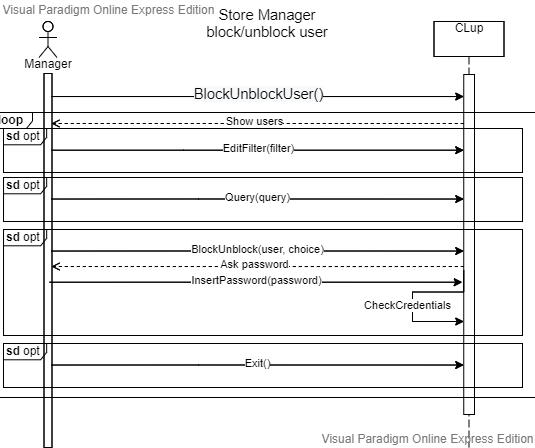
\includegraphics[width=\linewidth]{../Diagrams/BlockUser.png}
	\caption{Sequence diagram: Manager (un)block user}
	\label{fig:BlockUser}
\end{figure}

%SEQUENCE 2
\begin{figure}[H]
	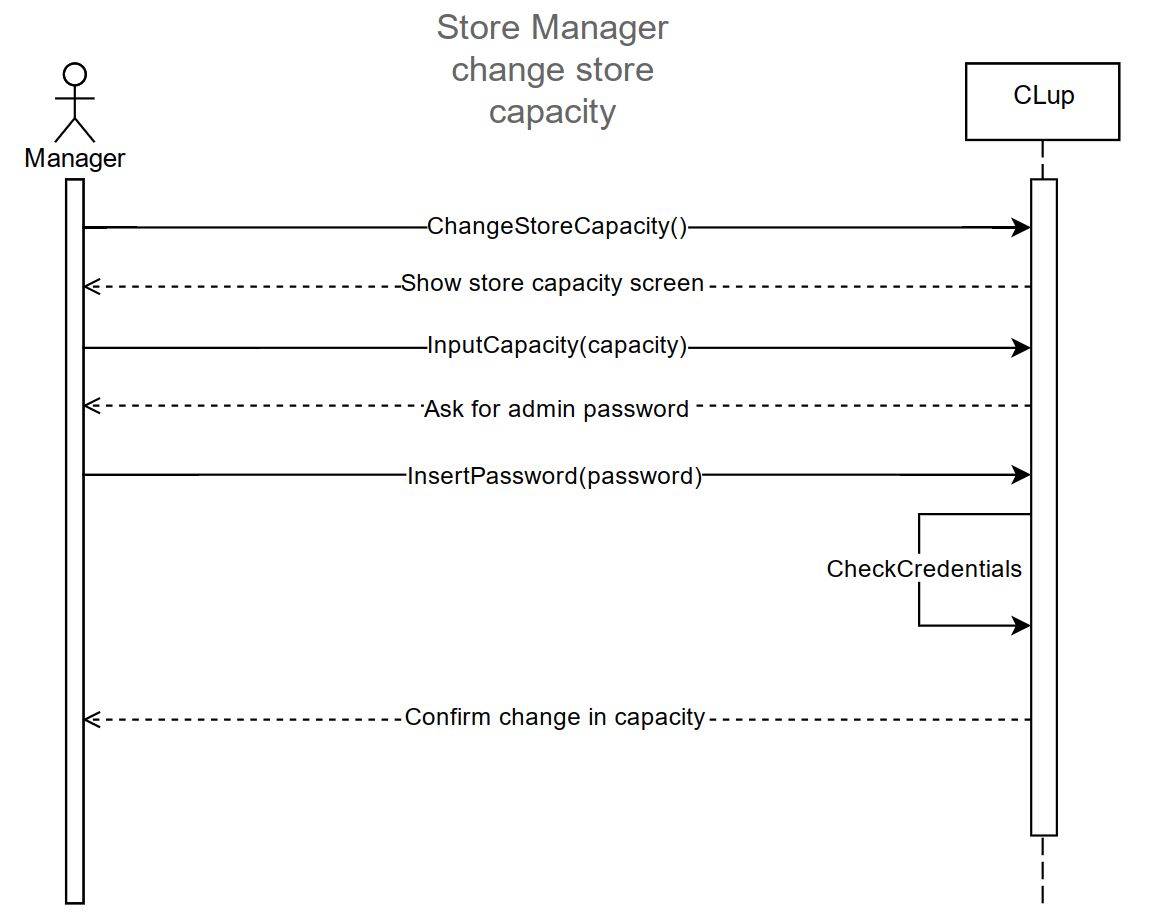
\includegraphics[width=\linewidth]{../Diagrams/ChangeCapacity.png}
	\caption{Sequence diagram: Manager changes capacity}
	\label{fig:ChangeCap}
\end{figure} 

%SEQUENCE 3
\begin{figure}[H]
	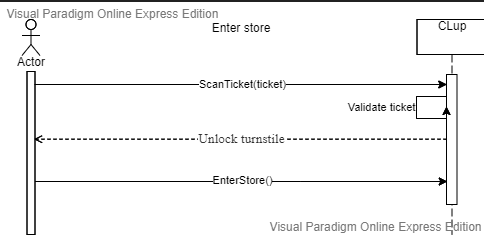
\includegraphics[width=\linewidth]{../Diagrams/EnterStore.png}
	\caption{Sequence diagram: Enter store}
	\label{fig:EnterStore}
\end{figure} 

%SEQUENCE 4
\begin{figure}[H]
	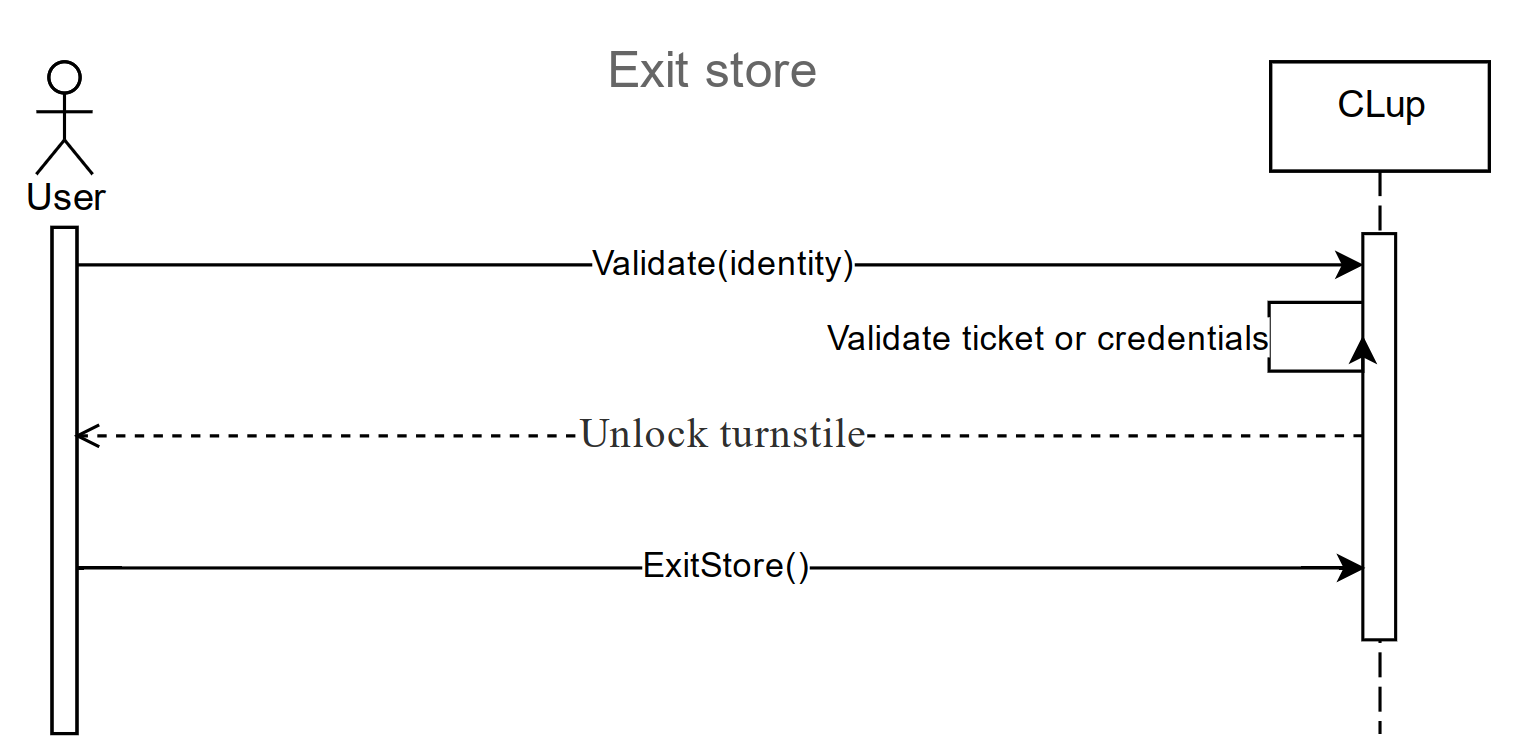
\includegraphics[width=\linewidth]{../Diagrams/ExitStore.png}
	\caption{Sequence diagram: Exit store}
	\label{fig:ExitStore}
\end{figure} 

%SEQUENCE 5
\begin{figure}[H]
	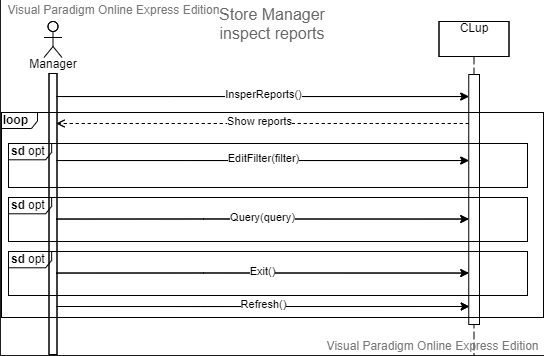
\includegraphics[width=\linewidth]{../Diagrams/InspectReports.png}
	\caption{Sequence diagram: Manager inspects report}
	\label{fig:InspectRep}
\end{figure} 

%SEQUENCE 6
\begin{figure}[H]
	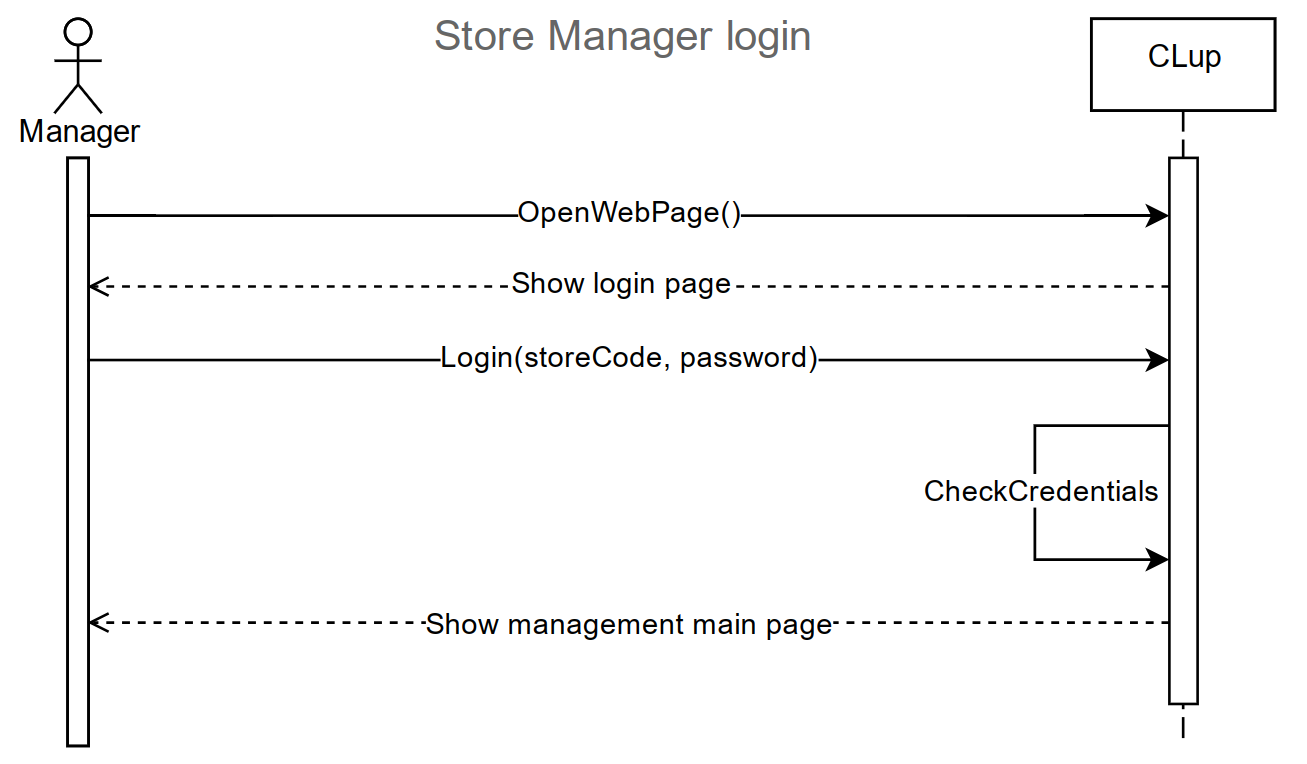
\includegraphics[width=\linewidth]{../Diagrams/ManagerLogin.png}
	\caption{Sequence diagram: Manager logs in}
	\label{fig:ManagerLog}
\end{figure} 

%SEQUENCE 7
\begin{figure}[H]
	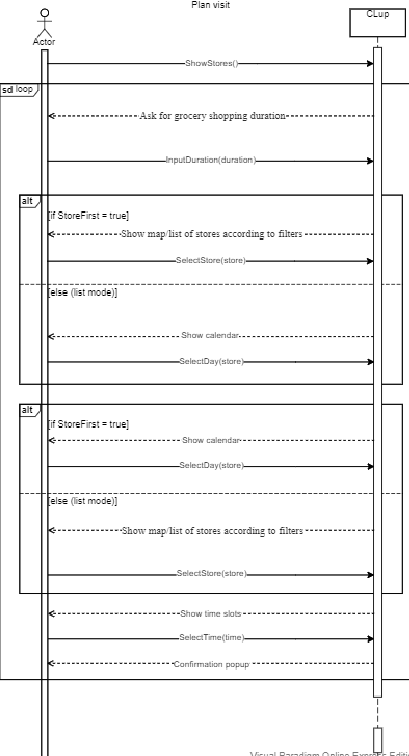
\includegraphics[width=\linewidth, height=22cm]{../Diagrams/PlanVisit.png}
	\caption{Sequence diagram: User plans visit}
	\label{fig:PlanVisit}
	%CERCA \scale
\end{figure} 

%SEQUENCE 8
\begin{figure}[H]
	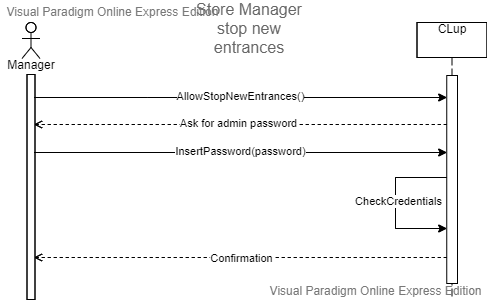
\includegraphics[width=\linewidth]{../Diagrams/StopEntrances.png}
	\caption{Sequence diagram: Manager stops entrances}
	\label{fig:StopEntr}
\end{figure} 

%SEQUENCE 9
\begin{figure}[H]
	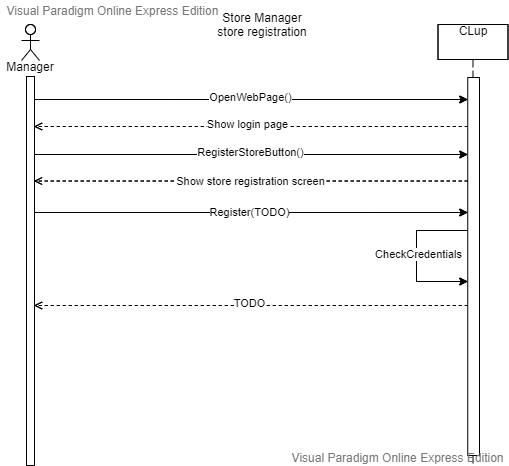
\includegraphics[width=\linewidth]{../Diagrams/StoreRegistration.png}
	\caption{Sequence diagram: Manager registers}
	\label{fig:StoreReg}
\end{figure} 

%SEQUENCE 10
\begin{figure}[H]
	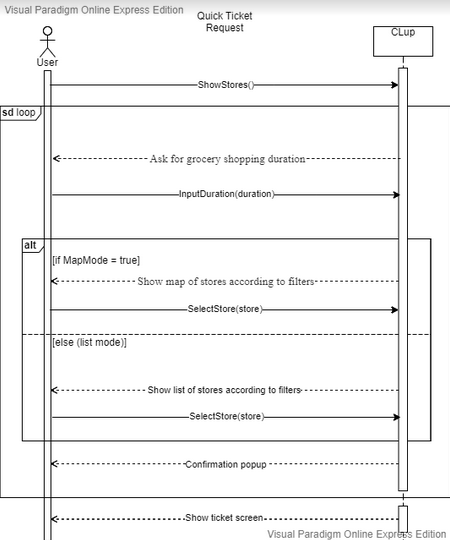
\includegraphics[width=\linewidth]{../Diagrams/TicketRequest.png}
	\caption{Sequence diagram: Quick ticket request}
	\label{fig:TicketReq}
\end{figure} 

%SEQUENCE 11
\begin{figure}[H]
	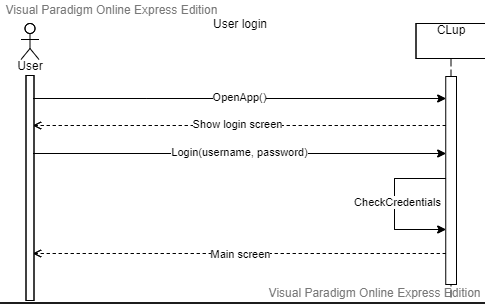
\includegraphics[width=\linewidth]{../Diagrams/UserLogin.png}
	\caption{Sequence diagram: User logs in}
	\label{fig:UserLog}
\end{figure} 

%SEQUENCE 12
\begin{figure}[H]
	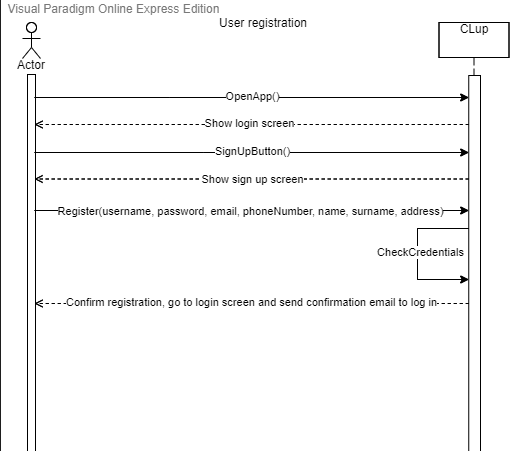
\includegraphics[width=\linewidth]{../Diagrams/UserRegistration.png}
	\caption{Sequence diagram: User registration}
	\label{fig:UserReg}
\end{figure} 

%SEQUENCE 13
\begin{figure}[H]
	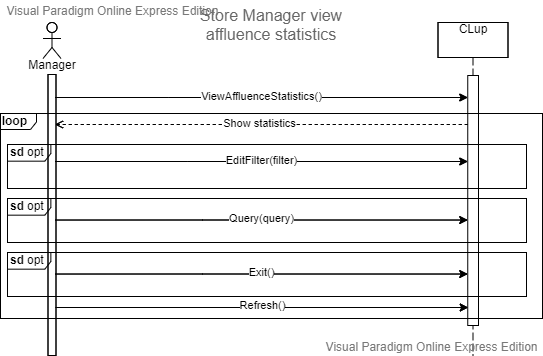
\includegraphics[width=\linewidth]{../Diagrams/ViewStatistics.png}
	\caption{Sequence diagram: Manager views customers statistics}
	\label{fig:Stat}
\end{figure} 

%SEQUENCE 14
\begin{figure}[H]
	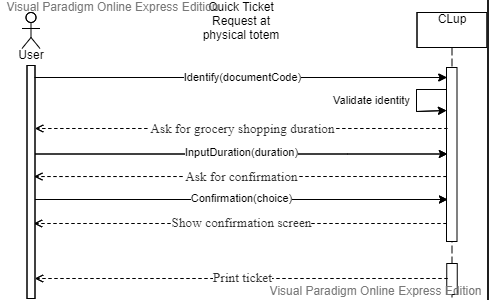
\includegraphics[width=\linewidth]{../Diagrams/Totem.png}
	\caption{Sequence diagram: Quick ticket at physical totem}
	\label{fig:Totem}
\end{figure} 


\subsection{Performance Requirements \label{subs:performance}}
Follows a list of critical performance conditions and their associated capabilities. \newline

\paragraph{Dynamic actions}
\label{par:dynamicActions}
Dynamic actions or changes that occur (e.g., rates, velocities, movements, and noise levels).
\begin{itemize}[leftmargin=+.8in]
    \item [\ref{par:dynamicActions}.1.1] CLup totems shall handle multi-touch recognition with a minimum of 2 concurrent points
\end{itemize}

\paragraph{Endurance capabilities}
\label{par:endurance}

Quantitative criteria covering endurance capabilities of the equipment required to meet the user needs
under stipulated environmental and other conditions, including minimum total life expectancy. Indicate
required operational session duration and planned utilization rate.
\begin{itemize}[leftmargin=+.8in]
    \item [\ref{par:endurance}.2.1] CLup totems shall run a minimum of 240 hours sessions between successive reboots
    \item [\ref{par:endurance}.2.2] CLup web application backend servers shall process a minimum of 10 requests per minute store-wise or alternative a minimum of 250K requests per minute country-wise
    \item [\ref{par:endurance}.2.3] CLup database servers shall process a minimum of 10K customer sign-up requests per minute, store-wise 
    \item [\ref{par:endurance}.2.4] CLup database servers shall process a minimum of 10 staff member sign-up requests per minute, store-wise
    \item [\ref{par:endurance}.2.5] CLup database servers shall handle a minimum of 100 customer-related queries per minute, store-wise
    \item [\ref{par:endurance}.2.6] CLup database servers shall handle a minimum of 10 staff-related queries per minute, store-wise
    \item [\ref{par:endurance}.2.7] CLup database servers shall handle a minimum of 10K bookings-related queries per minute, store-wise.
    \item [\ref{par:endurance}.2.8] CLup web application backend servers shall process a minimum of 10 login sessions per minute, store-wise 
    \item [\ref{par:endurance}.2.9] CLup web application servers shall cover a minimum expected lifetime of 5 years each
    \item [\ref{par:endurance}.2.10] CLup core servers shall cover a minimum expected lifetime of 5 years each
    \item [\ref{par:endurance}.2.11] CLup outside totems shall cover a minimum expected lifetime of 2 years each
    \item [\ref{par:endurance}.2.12] CLup outside totems shall withstand a minimum usage rate of 30 quick-ticket generations per hour, or 720 generations per day
    \item [\ref{par:endurance}.2.13] CLup outside totems shall withstand a minimum ticket generation session of 2 minutes
    
\end{itemize}

\paragraph{Performance requirements for operational phases}
\label{par:operationalPhases}

Performance requirements for the operational phases and modes.

\subsection{Design Constraints}
Follows a set of constraints on the system design imposed by external standards, regulatory requirements, or project
limitations.

\subsubsection{Standards compliance}
\label{standards}
The application requires adhesion to the following security standards:\newline 
\begin{itemize}
    \item Transport Layer Security standard (TLS) version 1.2 (or higher), \href{https://tools.ietf.org/html/rfc5246}{RFC 5246}
    \item Advanced Encryption Standard with a 128-bit key or more, \href{http://www.networksorcery.com/enp/rfc/rfc3394.txt}{RFC 3394}
\end{itemize}

\subsubsection{Hardware limitations}
As far as the app version is concerned, CLup \textbf{requires} a device with the following hardware to be operational:\newline
\begin{itemize}
    \item GNSS (any)
    \item screen
    \item pointing input device, such as touchscreens or mice
    \item internet connectivity
    \item audio output device
\end{itemize}

\bigskip \noindent Concerning the \textbf{reduced version} to be run on totems outside the stores, the following hardware is \textbf{requested}:\newline
\begin{itemize}
    \item screen
    \item pointing input device, such as touchscreens or mice
    \item internet connectivity
    \item printer device
\end{itemize}

\bigskip \noindent Finally, the web application for internal use requires: \newline
\begin{itemize}
    \item screen
    \item pointing input device, such as touchscreens or mice
    \item internet connectivity
\end{itemize}


\subsubsection{Any other constraint}
\paragraph{Environmental Constraints}
\label{par:envConstraints}
\begin{itemize}[leftmargin=+.8in]
    \item[\ref{par:envConstraints}.1.1] CLup totems shall withstand temperatures between -20$^{\circ}$ C and +50$^{\circ}$ C
    \item[\ref{par:envConstraints}.1.2] CLup totems shall withstand winds below 50 km/h
    \item[\ref{par:envConstraints}.1.3] CLup totems shall withstand relative humidity of at least 95\% 
\end{itemize}

\subsection{Software System Attributes}

\subsubsection{Reliability}
Given the presence of 24/7 stores, as additionally specified inside the Alloy Specification sect. (\ref{sect:alloy}), the system must have a guaranteed uptime of 24 hours a day, 7 days a week.
\subsubsection{Availability}
CLup targets the broadest group of individuals possible, given it's aimed at use for everyone as in depth explained in the previous sections. This indeed strains the availability constraints over the application which must be:\newline
\begin{itemize}
    \item available to people living inside slow connection areas, thus requiring a minimum 100Kb/s bandwidth to be operational
    \item available to old and/or low-end devices, being operational on a minimum configuration of:
    \begin{itemize}
        \item Android version 5.0 or higher
        \item 1.5 GHz dual core CPUs for Android devices
        \item 50 MBytes of minimum available storage memory for Android devices
        \item 512 MBytes of minimum system memory for Android devices
        \item iOS version 8.0 or higher
    \end{itemize}
    \item The staff-operations web application must be able to operate on any modern, HTML5 compliant web-browser, OS-independently 
\end{itemize}
{\color{gray}
\fbox{%
    \parbox {\textwidth}{%
        \small
        No support for deprecated, unsupported operating system (such as Microsoft \textregistered \space Windows Phone \textregistered) is being required as the overall market share of those system is below 0.1\%

    }%
}}


\subsubsection{Security}
CLup does not require best-in-class security measures given the mainstream nature of its main objectives, yet requires standard security measures to guarantee the following requirements:\newline
\begin{itemize}
    \item User data AES-128 (or stronger) encryption over the entire user database, as per sect. \ref{standards}
    \item Connection encryption between clients and servers to guarantee authentication and integrity 
    \begin{itemize}
        \item Transport Layer Security version 1.2 or higher, as per sect. \ref{standards}
    \end{itemize}
    \item Strong 2-factor authentication (or stronger) must be required for Staff operations, as they imply non-negligible consequences on store operativeness and availability to end users.
    \item Keep 6+ months old logs about internal staff operations and related authentication sessions.
    \item Application-level (or more) firewall over database and staff-operations related applications.
    \item Implementation or outsource use of \textit{anti-DoS} (Denial of Service) techniques/software components.
\end{itemize}

\subsubsection{Maintainability}
CLup is inevitably open to great expansion and innovation opportunities due to its potential broad use, hence the need for a highly maintainable and scalable system.
The following aspects are necessarily required:\newline
\begin{itemize}
    \item Code modularity
    \item Manual code writing privileging over automated generation, eventually privileging code maintainability and stability over eye-candiness and \textit{nice-to-haves} richness.
    \item Accurate and up-to-date documentation, with a maximum 5\% of already implemented,undocumented code rate over total
    \item Long term support software development kits usage
    \item Long term support external services usage
\end{itemize}


\subsubsection{Portability}
Given its broad spectrum target, CLup needs to be operational on the largest number of device/operating system configurations possible. Virtually no device should be eligible for no support by CLup, however this would potentially lead to infeasibility issues, ultimately slowing down or inhibiting CLup development. \newline
Therefore, the following minimum requirements are requested for maximised portability:\newline
\begin{itemize}
    \item A maximum of 10\% host-dependant code
    \item A maximum of 20\% elements based on host-dependant code
    \item Use of HTML5 for static web content
    \item Use of CSS for web styling
    \item Use of Java or C++ or C for core application functionalities
    \item Use of PHP for web application backends
    \item Use of Linux/Unix based OSs on all servers and end-user totems
    \item No use of Adobe \textregistered \space Flash \textregistered \space technologies
\end{itemize}

